% !TEX TS-program = xelatex
% !TEX encoding = UTF-8

\documentclass[12pt]{article}

\usepackage{fontspec} % Font selection for XeLaTeX; see fontspec.pdf for documentation
\defaultfontfeatures{Mapping=tex-text} % to support TeX conventions like ``---''
\usepackage{xunicode} % Unicode support for LaTeX character names (accents, European chars, etc)
\usepackage{xltxtra} % Extra customizations for XeLaTeX

\usepackage{geometry} % See geometry.pdf to learn the layout options. There are lots.
\geometry{a4paper, left=25mm, right=25mm, top=25mm, bottom=25mm} % or letterpaper (US) or a5paper or....
\usepackage[parfill]{parskip} % Activate to begin paragraphs with an empty line rather than an indent

\usepackage{graphicx} % support the \includegraphics command and options

\usepackage{listings}
\lstset{basicstyle=\ttfamily,columns=fullflexible,keepspaces=true}

%%%%%%%%%%%%%%%%%%%%%%%%%%%%%%%%%%%%%%%%%%%%%%%%%%

\title{Report 4: Threads}
\author{Dinh Ngoc Tu}

\begin{document}
\maketitle

%%%%%%%%%%%%%%%%%%%%%%%%%%%%%%%%%%%%%%%%%%%%%%%%%%

\section{Implementation}

First, we calculated the dimension of the picture, and the dimension of the grid:

\begin{lstlisting}[breaklines]
int blockSize = ...;
long gridWidth = (inputImage->width + blockSize - 1) / blockSize;
long gridHeight = (inputImage->width + blockSize - 1) / blockSize;
dim3 gdim(gridWidth, gridHeight);
dim3 bdim(blockSize, blockSize);
\end{lstlisting}

The remaining host code is the same as before.

The CUDA code is implemented as follows:

\begin{lstlisting}[breaklines]
__global__ void labwork4(uchar3 * __restrict__ input, uchar3 * __restrict__ output, long long pixelCount, int width) {
    long row = blockIdx.y * gridDim.y + threadIdx.y;
    long long i = row * width + threadIdx.x;
    if (i < pixelCount) {
        output[i].x = (char)(((int)input[i].x + input[i].y + input[i].z) / 3);
        output[i].y = output[i].z = output[i].x;
    }
}
\end{lstlisting}

The code first calculates the row index in the image, then the pixel position. Finally, it calculates the output pixel value.

%%%%%%%%%%%%%%%%%%%%%%%%%%%%%%%%%%%%%%%%%%%%%%%%%%

\section{Speedup}

The speedup is as follows:

\begin{figure}[h]
    \centering
    \caption{Speedup with CUDA}
    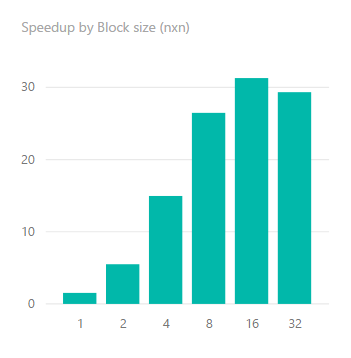
\includegraphics{pics/lw4.png}
\end{figure}

As shown on the graph above, the speedup given by CUDA is anywhere from 1.5x to 31x depending on block size, and increases quickly
until a blocksize of $8 \times 8$. A block size of $16 \times 16$ gives the highest performance.

%%%%%%%%%%%%%%%%%%%%%%%%%%%%%%%%%%%%%%%%%%%%%%%%%%

\section{Exercises}

\begin{enumerate}
    \item $16 \times 16$, since $16 \times 16 = 256 < 512$ threads/block; the SM can therefore fit 4 blocks into the SM and run at full capacity.
          With $8 \times 8$, we need 16 blocks to fill the SM, but the SM only supports 8 blocks at once.
          With $32 \times 32$, each block has 1024 threads; therefore, we go over the thread limit in each block.
    \item 512, since with 512 threads per block and a maximum of 4 blocks, the SM can take 3 blocks and run 1536 threads for full capacity.
          With 128/256/1024 threads per block, you can only run 512/1024/1024 threads on the SM concurrently, respectively.
    \item We use 4 blocks for a total of $4 \times 512 = 2048$ threads.
\end{enumerate}

%%%%%%%%%%%%%%%%%%%%%%%%%%%%%%%%%%%%%%%%%%%%%%%%%%

\end{document}